\Chapitre{Raccordement}

\section{Principe}

Les réseaux sont constituer de groupe de modules. 
Aux extrémités de ces groupe, se trouve une interface de raccordement standard. 
De cette manière les groupe sont interchangeable. 
Mais les modules à l'intérieur de ces groupes ne le sont pas forcément. 

Les interfaces à l'interne des groupes de modules correspondent aux interfaces standard sauf pour l’emplacement de la voie et le décors.

\section{Interface standard}

Les interfaces standard correspondent au dessin suivant.

Sur les modules de plus de 400mm de large, l'axe de la voie est pris comme référence.
L'axe de la voie doit être au minimum à 200mm du bord du module.

Les interfaces standard sont à des hauteurs définies.
% TODO préciser les hauteurs exactes des interfaces standard

\subsection{Protection voie}

Si des protections pour la voie sont prévues, elles doivent suivre le dessin correspondant.
% TODO faire le dessin

\section{Raccordement électrique}

Les modules de pleine voie sont équipés de 2 bus d'alimentation : l'alimentation traction pour la voie et une alimentation pour les accessoires.

Sur le module vue de face,

Les fils doivent être suffisamment long pour se connecter à une prise sur le module voisin à 200mm du bord avec un rebord de 100mm.

Si le rebord du module est plus haut que 100mm un trou doit être fait pour passer les fils.

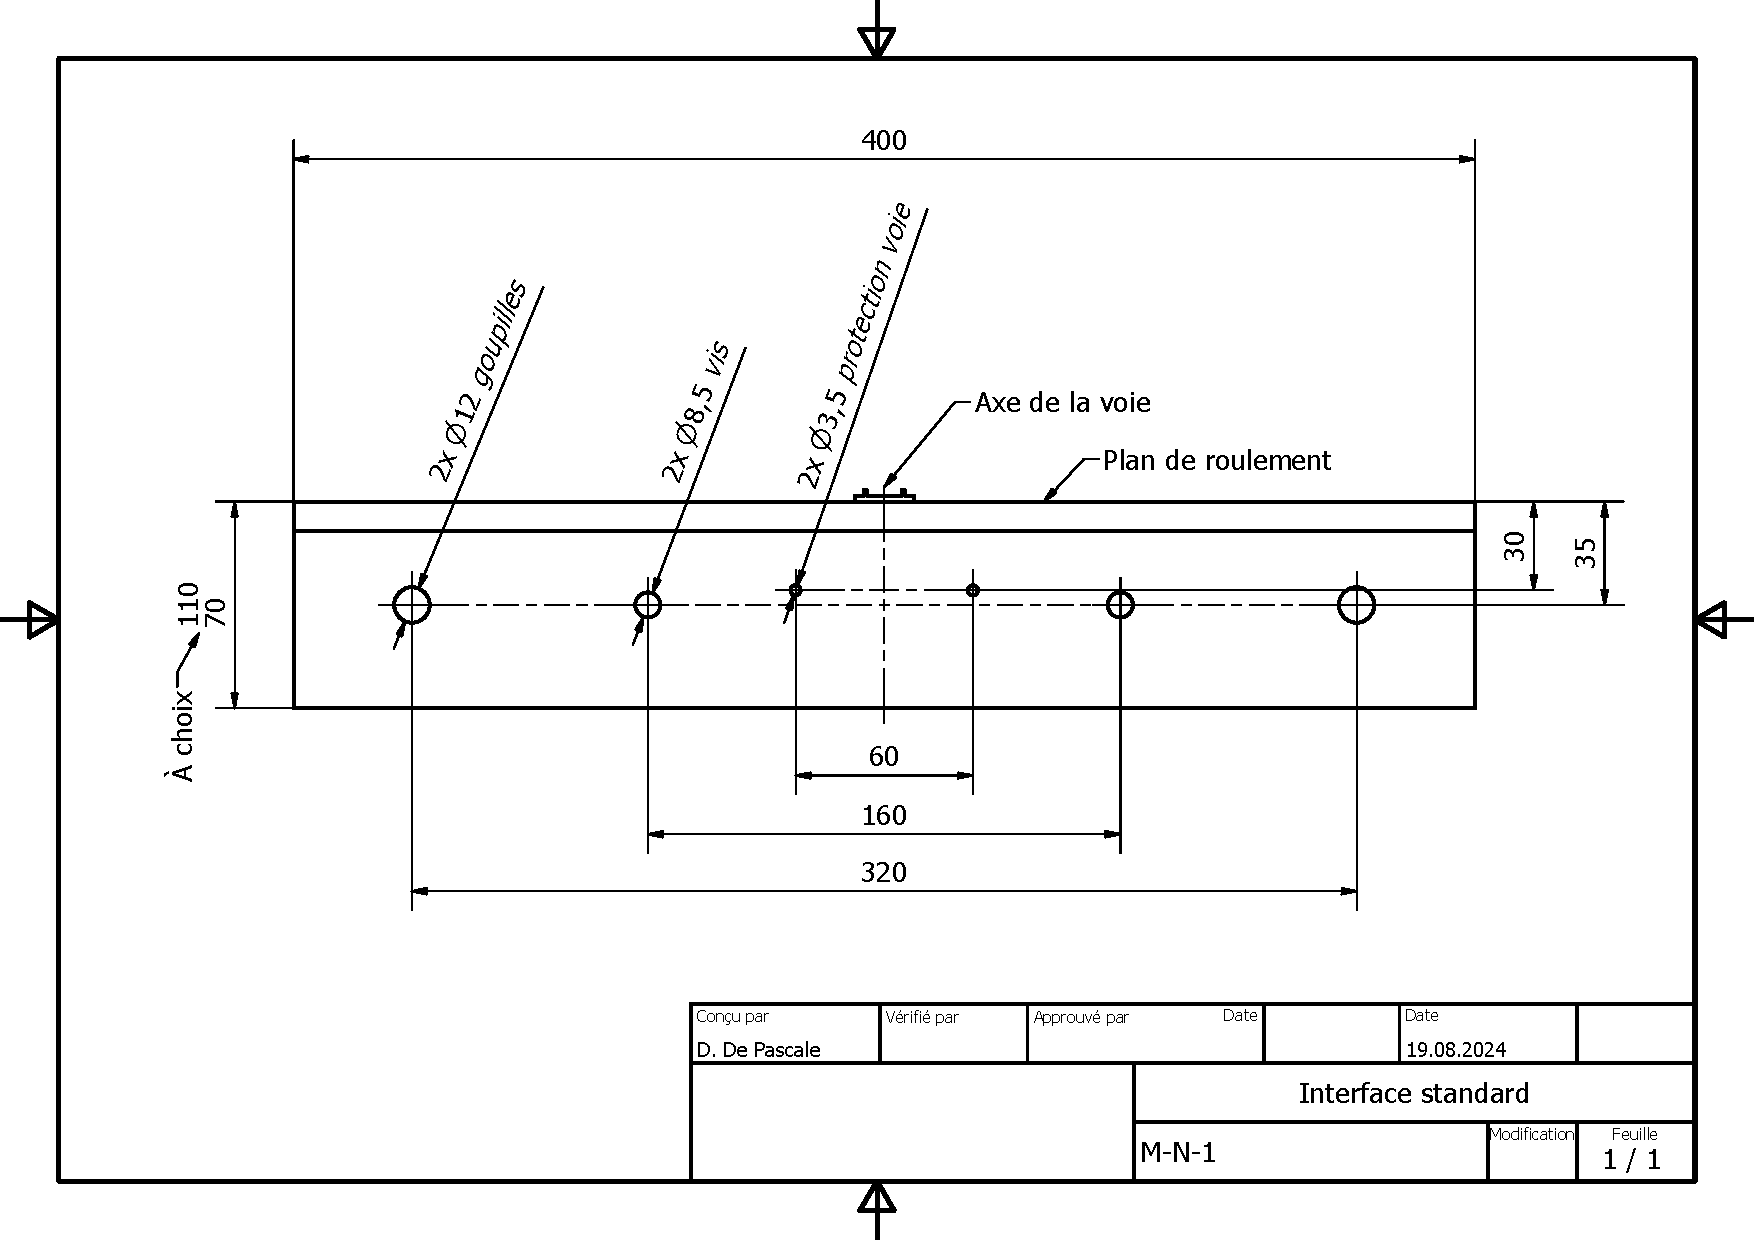
\includepdf[pages=-, fitpaper=true]{images/mecanique/M-N-I40.pdf}
% TODO remplacer "plan de roulement" par le bon nom.